\documentclass[french]{article}
\usepackage[utf8]{inputenc}
\usepackage[french]{babel}
\usepackage[T1]{fontenc}
\usepackage{babel}
\usepackage{amsmath,trimclip}
\usepackage{graphicx}
\usepackage{hyperref}
\usepackage{mathtools}
\usepackage{array}
\usepackage{biblatex}
\usepackage{algorithm}
\usepackage{algpseudocode}
\usepackage{siunitx}
\usepackage[strings]{underscore}
\addbibresource{biblio.bib} 


\title{Test de propriétés et BDD}
\author{Alpha DIALLO, Lamine KEITA, Sacha MEMMI}
\date{Avril 2020}



\begin{document}


\maketitle
\begin{figure}[htp]
    \centering
    
\includegraphics[width=5cm, height=2cm]{logo_upmc}
    \label{fig:logo}
\end{figure}

\begin{large}
\begin{center}
    Encadrant: Antoine Genitrini
\end{center}
\vfill
\begin{flushright}
\text{Université Pierre et Marie Curie}\medskip

\text{Paris, France}\medskip

\text{Pstl}\medskip

\text{Master 1, Semestre 2}
\end{flushright}
\end{large}


\newpage
\tableofcontents
\newpage
\section{Abstract}

Les fonctions booléennes sont très largement utilisées en science. Elles sont aussi largement utilisées parce que simple à manipuler et à mettre en place leur utilité est également très large. On les utilise par exemple en électronique pour travailler sur les circuits logiques.
\vspace{5mm} 

Les structures avec lesquelles nous travaillons dans ce rapport sont ce que l'on appelle des robdd, Reduced Ordered Binary Decision Diagram. Elles représentent les fonctions booléennes en tant que graphes (dirigés et acycliques). Elles sont l'une des méthode préférée pour représenter celles-ci, en particulier, en informatique. Elles sont préférées car facile à implémenter, quelques ligne de codes dans n'importe quel langage sont suffisantes pour les représenter, mais également parce qu'elles sont simples à manipuler.
\vspace{5mm} 

En particulier nous cherchons à énumérer le nombre de robdd unique représentant une fonction ayant un nombre défini de variables selon leur taille. Ce problème a intéressé le domaine scientifique depuis que ces structures ont vu le jour, il présente de nombreux intérêts dans tous les domaines où l'on travail avec des robdd.
\vspace{5mm} 

En plus de rappeler la méthode standard de génération des robdd, nous donnerons un moyen de reconstruire ces structures. Nous obtenons par cette nouvelle méthode un générateur uniforme de robdd que nous pouvons insérer dans des outils tels que Quickcheck, outil au sujet duquel nous consacrerons un chapitre dans ce rapport. 

\begin{figure}[h!]
    \centering
    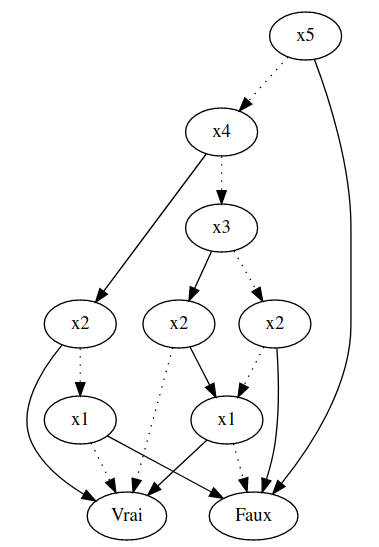
\includegraphics[scale=0.4]{robdd de presentation.png}
    \caption{Robdd généré avec la méthode du unranking}
    \label{fig:ROBDD1}
\end{figure}
\newpage
 Avec notre méthode, nous avons pu générer le robdd de taille 10 sur 5 variables de la figure \ref{fig:ROBDD1}.
 
 La méthode de génération de robdd présenter dans ce rapport s'appuie sur celle présenter dans \cite{genitrini}, en plus d'implémenter en pseudo-code des algorithmes introduits dans ce papier nous en fournissons certains non décrits dans celui-ci.



\section{Introduction}
L'idée derrière les arbres de décisions binaires a été introduite par Shannon en 1938 dans \cite{shannon}. C'est en 1959 que Lee introduit l'idée de bdd dans \cite{lee}.

Les diagrammes de fonction binaires sont principalement des outils pour les ingénieurs (et autre professions travaillant dans le hardware en informatique) qui manipulent des circuit électroniques, cas où l'utilisation de tables de vérité se révèle efficace. Dans ce cas là, diviser leur circuit complexe en sous circuits simples comme le permettent les diagrammes de décisions binaires (concept que l'on appelle "diviser pour régner") est très efficace.\medskip

Plus particulièrement, les circuits électroniques sont devenus si compliqués que les robdd sont à peine suffisants pour les traiter comme l'a noté Knuth il y a de ça plus de 10 ans \cite{knuth}. \medskip

Un bdd (binary decision diagram) est un diagramme de décision binaire pouvant représenter une fonction booléenne. Il est important de souligner que l'utilisation des BDD est bien plus vaste que la seule application aux fonctions booléennes. Cependant, nous nous concentrerons sur celles-ci durant cette étude. Nous pouvons voir un exemple de BDD, celui de la figure 2 peut être utilisé pour représenter la fonction booléenne : \(\Bar{x3}(x2+\Bar{x3})+x3(\Bar{x2}+x1)\) , ainsi que la table de vérité ci dessous:
\vspace{5mm} 

\begin{tabular}{llll}
  \hline
  x_3 & x_2 & x_1 & R \\
 \hline
  $\bot$ & $\bot$ & $\bot$ & $\top$ \\
  $\bot$ & $\bot$ & $\top$ & $\top$ \\
  $\bot$ & $\top$ & $\bot$ & $\top$ \\
  $\bot$ & $\top$ & $\top$ & $\bot$ \\
  $\top$ & $\bot$ & $\bot$ & $\bot$ \\
  $\top$ & $\bot$ & $\top$ & $\top$ \\
  $\top$ & $\top$ & $\bot$ & $\top$ \\
  $\top$ & $\top$ & $\top$ & $\top$ \\
  \hline
\end{tabular}
\vspace{5mm} 

Un robdd (reduced ordered binary decision diagram) est comme son nom l'indique la forme réduite et ordonnée d'un bdd. Dans la littérature le terme bdd est presque toujours utilisé pour évoquer un robdd, nous ferons d'abord la distinction entre ces deux termes pour mettre l'accent sur l'aspect réduction. Les bdd que nous considérons dans ce rapport sont toujours ordonnés. Dans cette étude, lorsque nous ferons parlerons de BDD, nous ferons référence aux obdd  (ordered binary decision diagrams).\medskip

Les robdd n'ont été introduit qu'en 1986 \cite{bryant_graph}. Assez tard dans l'histoire de l'informatique. Les robdd ont été une telle révolution que \cite{bryant_graph} est pendant des années resté le rapport le plus cité en science de l'informatique comme l'a noté Knuth:

\begin{center}
    \emph{"His (Randal E. Bryant's) introduction to the subject [IEEE Trans. C-35 (1986),677-691] became for many years the most cited papers in all of computer science"}\cite{knuth}
\end{center}

De nombreuses autres variantes de robdd ont également été créées depuis \cite{wegner}.\medskip

Le principe d'un robdd est simple, on cherche à conserver de l'espace mémoire en se débarrassant des structures redondantes, la mémoire étant une préoccupation importante en informatique. Pour réduire un bdd, nous supprimons les sous structures redondantes, nous supprimons également les noeuds non essentiels. Nous représentons les bdd en tant qu'arbre plat et les robdd en tant que DAG (directed acyclic diagrams) \cite{flajolet_automata}. Plus généralement, les robdd sont des sous types de bdd et tous les types de bdd peuvent être représentés par un dag.\medskip

\begin{center}
\emph{“A function in Boolean algebra. The function is written as an expression formed with binary variables (taking the value 0 or 1) combined by the dyadic and monadic operations of Boolean algebra.”} 
\end{center}

- Oxford Reference 
\vspace{5mm} 

Il existe de nombreux moyens pour représenter des fonctions booléennes. Ceux préférés en science de l'informatique sont les diagrammes, pas seulement grâce à la manière dont ces diagrammes peuvent être réduits, mais aussi parce qu'ils peuvent être conservés en mémoire en tant que suites de noeuds qui ne sont pas forcement adjacents en mémoire les uns par rapport aux autres. Ceci rend leur conservation plus simple et efficace.

\begin{figure}[h!]
    \centering
    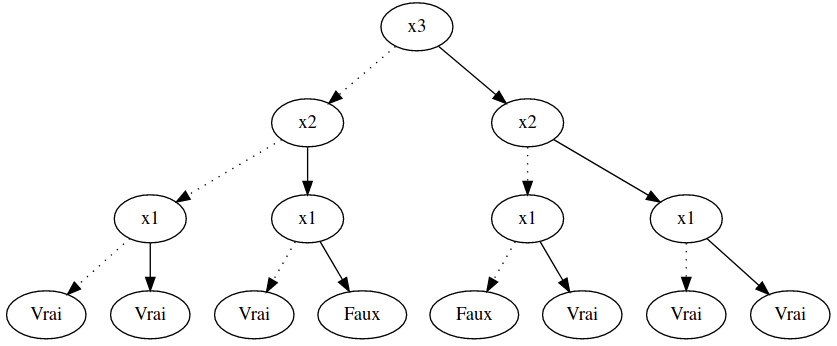
\includegraphics[scale=0.4]{bdd ex1.png}
    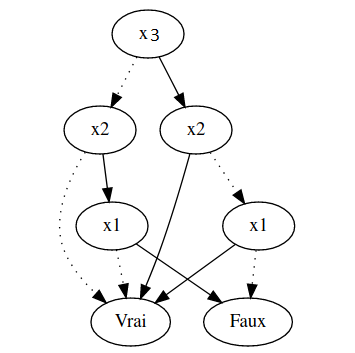
\includegraphics[scale=0.4]{robdd ex1.png}
    \caption{Arbre de decision binaire en haut et dag représentant sa forme réduite en bas}
    \label{fig:ROBDD1}
\end{figure}
\vspace{5mm} 

Un exemple d'arbre de décision binaire et un DAG représentant sa forme réduite sont donné dans la figure \ref{fig:ROBDD1}. Nous suivons ici le consensus dans la littérature et représentons les liens vers les fils haut par une ligne solide, et ceux vers les fils bas par une ligne en pointillé. Le fils haut (respectivement fils bas) d'un noeud est le noeud successeur de celui marqué par un arc 1 (respectivement 0), la valeur de transition vers ce noeud dans la fonction de transition est donc 1 (respectivement 0).\medskip

En plus de l'utilité évidente des fonctions booléennes ont peut aussi noter que les bdd sont devenus aussi populaires, car comme Knuth l'a noté dans \cite{knuth}, les bdd simples sont relativement facile à fusionner pour obtenir des bdd plus complexes.\medskip

Dans ce rapport notre but est de présenter un nouveau procédé permettant d'énumérer des robdd sans passer par le processus de compression, procédé introduit dans \cite{genitrini}.\medskip

Le processus de compression est relativement simple avec une complexité polynomiale, mais la méthode standard de génération des bdd d'un nombre donné de variables k utilisé jusqu'ici était impraticable pour {\(k > 4\)} \cite{newton}. Pour construire les bdd ayant k variable dans la méthode standard nous construisons tout d'abord toutes les fonctions booléennes ayant k variables, puis leurs bdd, puis compressons ces bdd afin d'obtenir leurs robdd et enfin nous supprimons les robdd apparaissant plus d'une fois. Ceci avait une complexité doublement exponentielle de  O(\( {2^2}^k\) ).\medskip

Nous définissons la taille d'un robdd par le nombre de noeuds internes (non terminaux) qu'il contient.

Pour énumérer ces structures dans la méthode que nous introduisons ici, nous utilisons de nombreuses propriétés des robdd.  Nous utilisons ensuite des méthodes dites de unranking et ranking basées sur le modèle standard introduit dans \cite{wilf} en définissant un ordre total sur les robdd et en décomposant chacun par une constitution de sous robdd.

Le processus de ranking consiste à attribuer à chaque objet d'un ensemble un identifiant unique. Celui du unranking consiste à retrouver, à partir d'un identifiant, un objet au d'un ensemble d'arbres possibles.\medskip

Nous obtenons grâce à cette méthode un générateur uniforme de robdd.\medskip

Avec la méthode standard utilisée dans \cite{newton} les robdd de taille proche de la taille maximale étaient crées avec une grande probabilité, mais dans celle ci chaque robdd a un identifiant unique dans l'ensemble. On peut également modifier ce générateur pour ne créer que des robdd ayant certains types de propriétés.

\begin{figure}[htp]
    \centering
    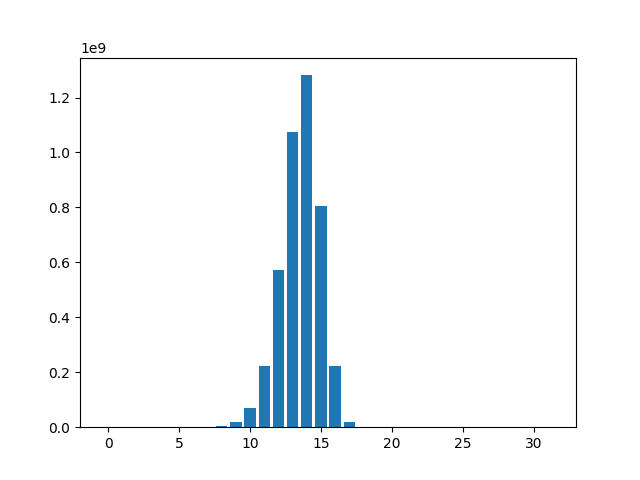
\includegraphics[width=9cm, height=6cm]{index5}
    \caption{Distribution des taille de bdd ayant 5 variable}
    \label{fig:Figure1.2}
\end{figure}

Avec notre méthode nous arrivons a comptabiliser les bdd ayant 5 variables, avec une implantation en python et un matériel limité, en 14 secondes.\medskip

En faisant une comparaison des résultats trouvés dans \cite{newton} et visibles sur la figure \ref{fig:Figure1.3} on remarque que nos résultats visibles sur la figure \ref{fig:Figure1.2} y sont similaires (on rappelle qu'ici on ne prend pas en compte les feuille dans le calcul de la taille d'un bdd).\medskip

\begin{figure}[htp]
    \centering
    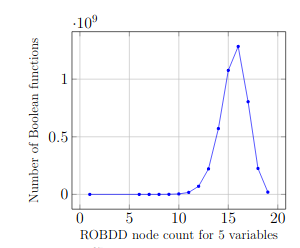
\includegraphics[width=6cm, height=5cm]{screen de newton.png}
    \caption{Distribution des taille de bdd ayant 5 variable selon \protect\cite{newton}}
    \label{fig:Figure1.3}
\end{figure}

Dans ce rapport nous considérerons que nous ne rencontrons jamais le robdd réduit au noeud unique \(\top\) ou \(\bot.\)
\newpage
\section{BDD et ROBDD}
Dans cette section nous cherchons à définir les structures basiques avec lesquelles nous travaillons, les bdd et les robdd.\medskip

Un bdd est composé de noeuds ayant un label. Chaque noeud non terminal possède deux enfants, ou fils, un bas et un haut liés à leurs parents par des liens notés respectivement 0 et 1. Chaque noeud a un index qui détermine son ordre dans le bdd. Les noeuds sont traités dans l'ordre décroissants de leur index.

La manière dont nous ordonnons les noeuds est importante comme noté dans \cite{newton} et trouver l'ordre le plus efficace est un problème NP (nondeterministic polynomial time).

La racine a un index k qui est l'index maximal de la bdd (ou robdd), et les noeuds terminaux ont des index nuls. Tous les noeuds internes (quand ils existent) ont des indexes allant de k à 0, non inclus. Pour un bdd l'index de la racine est le nombre de variables de la fonction booléenne qu'il représente, pas forcement pour un robdd.\medskip

Un bdd associe à chaque affectation de variables une valeur de retour, pour connaître cette valeur nous allons tout d'abord à la racine, puis nous suivons un chemin en se fiant à la valeur de chaque variable données en entrée selon l'index du noeud courant. Si la variable d'index du noeud courant est 0 nous nous rendons à l'enfant bas du noeud courant, l'enfant haut si la variable a pour valeur 1. Nous finissons par arriver à un noeud terminal, que dans le reste de ce rapport nous appellerons feuille, de valeur \(\top\) (true) ou \(\bot\) (false) qui est la valeur de retour de la bdd pour les variables considérées.

Pour un bdd, de la figure \ref{fig:ROBDD1} si l'on donnait les variables 101 en tant qu'entrée elle retournerait \(\top\) (true). 

La méthode classique pour obtenir un robdd est de réduire un arbre de décision binaire. 

Pour effectuer cette réduction nous suivons tout d'abord deux règles, que nous notons R et M.
\vspace{5mm} 

Considérons \(\Delta\) un dag représentant une fonction booléenne f. Considérons également \(\alpha\) et \(\beta\)  deux noeuds distincts dans \(\Delta\) .

\textbf{Règle M}: Si \(\alpha\) et \(\beta\) sont des racine des sous graphes isomorphes alors fusionner \(\beta\) et \(\alpha\).

\textbf{Règle R}: Si les deux fils de \(\beta\) sont isomorphes à \(\alpha\), alors faire pointer tous les liens entrant de \(\beta\) vers \(\alpha\) et supprimer \(\beta\).

Nous appliquons récursivement ses deux règles à tous les noeuds de \(\Delta\) .
\vspace{5mm} 
\newpage
Deux ordres de parcours peuvent être considérés, \(post_{o}\) et \(pre_{o}\).

Dans l'ordre de parcours \(post_{o}\) nous visitons tous d'abord le fils bas du noeud courant, puis son fils haut et enfin le noeud lui-même.
Dans l'ordre de parcours \(pre_{o}\) nous visitons tous d'abord le noeud courant, puis son fils bas, et enfin son fils haut.

Nous choisissons ici de considérer l'ordre de traversée \(post_{o}\) pour effectuer chacune de nos compressions, puisque c'est celui préféré en science de l'informatique. Choisir un ordre en particulier est important pour s'assurer que des bdd équivalents soient compressés en tant que robdd identique une fois l'ordre des variables établie.
\vspace{5mm} 

Nous pouvons désormais définir formellement le processus de compression.

\textbf{Compression} :  Considérons \(\Delta\) le bdd de la fonction f.  Quand le noeud \(\lambda\) est visité, \(\lambda\) étant l'enfant d'un noeud \(\mu\). Si un sous-arbre \(\Lambda\), celui qui a pour racine \(\lambda\), a déjà été vu lors de la traversée de \(\Delta\), sous arbre dont la racine est \(\omega\), alors \(\Lambda\) est supprimé de \(\Delta\) et le noeud \(\mu\) obtient un pointeur vers \(\omega\), remplaçant le lien allant précédemment de \(\mu\) à \(\lambda\). Une fois la traversée de \(\Delta\) achevée, le DAG résultant est le robdd de f.
\vspace{5mm} 

Définissons maintenant formellement un robdd, cette définition ainsi que les notations que l'on utilise se basent sur celles définies dans \cite{genitrini}.

Considérons un robdd \(\Delta\) = (Q, I, r, \(\delta\)). Q est l'ensemble de noeuds que l'on obtient par une traversé en \(post_{o}\) de \(\Delta\). r est la racine de \(\Delta\), I est la fonction qui associe pour tout noeud \(\lambda\) \(\in\) Q son index et \(\delta\) est la fonction de transition complète qui associe à chaque noeuds ses fils.
\begin{itemize}
    \item
    	Q  =   ([feuille1],[feuille2], …, r)
    	([feuille1] etant la premiere feuille que l'on rencontre lorsque l'on parcourt \(\Delta\) en \(post_{o}\) et [feuille2] la seconde)
    \item 
        \(I = Q   \rightarrow  \{0, \ldots , k\}\) où k est l'index de r
    \item 
       \( \delta = (Q \setminus  \{\top,  \bot\}) * \{0, 1\} \rightarrow \) Q
\end{itemize}

On note que Q a une taille forcément supérieure ou égale à 3.

On peut ainsi representer le dag de la figure \ref{fig:ROBDD1} par un robdd \(\Delta\) = (Q, I, r, \(\delta\)) ayant les propriétés suivantes:
\begin{itemize}
    \item
    	Q  =   \((\bot, \top, x1,x1,x2,x2,x3)\)
    \item 
        \(I = \{\bot, \top, x1,x1,x2,x2,x3\}   \rightarrow  \{0,0,1,1,2,2,3\}\)
    \item 
       \( \delta = \{ x1 * 0 \rightarrow \bot , x1 * 1 \rightarrow \top, x1 * 0 \rightarrow \top , x1 * 1 \rightarrow \up, x2 * 0 \rightarrow x1, x2 * 1 \rightarrow \top, x2 * 0 \rightarrow \top, x2 * 1 \rightarrow x1, x3 * 0 \rightarrow x2, x3 * 1 \rightarrow x2 \} \) Q
    \item 
        r = x3
\end{itemize}

Dans le reste de ce rapport nous utiliserons le terme bdd pour faire référence aux robdd.
\newpage
\section{(RO)BDD : propriétés}
Dans cette section nous définissons des propriétés que l'on assigne aux bdd. Pour ce faire, nous mettons en place un ensemble de notations et d'opérations. Toutes les notations utilisées dans cette section seront utilisées dans le reste de ce rapport. Les opérations que nous définissons pour les listes sont également applicables aux ensembles. On se contente ici de redéfinir les notations définies dans \cite{genitrini}.
\vspace{5mm} 

Pour deux noeuds \(\alpha\) et \(\beta\) d'un dag \(\Phi\) nous écrivons \(\alpha\) \(\Leftarrow_{post}\) \(\beta\) si le noeud \(\alpha\) est visité avant le noeud \(\beta\) en \(post_{o}\) lors de la traversée de \(\Phi\), et \(\alpha\)\(\Leftarrow_{pre}\) \(\beta\) si le noeud \(\alpha\) est visité avant le noeud \(\beta\) en \(pre_{o}\) lors de la traversée de \(\Phi\).
\vspace{5mm} 

Pour deux listes l et l’ de tailles respectives m et n, où l = (p0,p1…,pm) et l’ = (p’0,p’1,…,p’n) nous écrivons L=l+l’ l'opération telle que si m\(<\)n avec L=(P0,P1,…,Pn) alors nous avons pour \(i\leq\) m Pi=pi+p’i et pour \(m<i\leq n\) Pi=p’i.

Pour une liste l nous notons \(\mid l\mid \) le nombre d'éléments dans l, et \(\mid\mid l\mid\mid\) la somme de tous ses éléments.
\vspace{5mm} 

\textbf{Profil d'un ensemble}: Le profil P=profil(S) d'un ensemble S est simplement une liste du nombre d'élément de S ayant un certain index, on note P = (p0,p1…,pj,…pk) où pj est le nombre d'éléments dans l'ensemble S d'index j et k l'index maximal de S. 

Le processus d'extension de cette définition de profil à des graphes est évident.
\vspace{5mm} 

\textbf{Squelette d'un bdd} : Considérons un bdd \(\Delta\) = (Q, I, r, \(\delta\)) enraciné en r. Le squelette T = (Q’, I, r, \(\delta\)’) de \(\Delta\) est un dag tel que Q’ = Q / \{\(\top,\bot\)\} où chaque noeud \(\lambda\) \(\in\) Q’ a été obtenu par la traversée en \(post_{o}\) de \(\Delta\) en faisant omission des deux feuilles. Les liens du squelette sont décrit en utilisant une fonction de transition partielle \(\delta\)’: Q’ \(\times\) \{0, 1\} \(\rightarrow\) Q' \(\cup\) \{nil\} où nil est un symbole spécial désignant une transition non définie.

Plus simplement, un squelette est un bdd auquel on retire les deux feuilles et les pointeurs.

Dans le reste de ce rapport nous nous référerons aux valeurs non définis de la fonction de transition partielle en tant que nil transition.
\vspace{5mm} 

Nous notons n le nombre de noeud d'un dag \(\Delta\) d'un bdd, nous savons que son squelette S a le même nombre de noeud que \(\Delta\) à l'exception des deux feuilles. Nous pouvons ainsi noter que S a (n-2) noeuds. Nous savons également que tous les noeuds non terminaux de \(\Delta\) ont deux enfants, ainsi le nombre de transition dans \(\Delta\) est (n-2)*2, ce qui est le nombre total de transition dans S (a la fois les transition nil et non nil). Nous savons également que chaque noeud \(\lambda\) \(\in\) S a nécessairement un degré entrant de 1 à l'exception de la racine. Ainsi le nombre restant de transitions non nil dans S est (n-3). Nous pouvons maintenant conclure que S a un nombre de nil transition égal à (n-1).
\vspace{5mm} 

\textbf{Sous arbre} : Un sous arbre TA(\(\lambda\)) est un arbre enraciné en \(\lambda\) appartenant à un autre arbre.

\textbf{Pool} : Considérons un dag D, la pool PT(\(\lambda\)) d'un noeud \(\lambda\) \(\in\) D est:

\begin{center}
PT(\(\lambda\)) = \{\(\tau\)’ \(\in\) D \(\mid\)  \(\tau\)’ \(\Leftarrow_{pre}\) \(\lambda\) et I(\(\tau\)’) \(<\) I(\(\lambda\))\} \(\cup\) \{\(\top\), \(\bot\)\} .
\end{center}

\textbf{Pool profil} : Le pool profil de \(\lambda\) est comme son nom l'indique le profil de sa pool que l'on note: profil(PT(\(\lambda\))). 

\textbf{Level set} : Considérons un dag D, le level set \(\lambda\) \(\in\) D est:
\begin{center}
ST(\(\lambda\)) = \{\(\theta\)’ \(\in\) D \(\mid\) \(\theta\)’ \(\Leftarrow_{pre}\) \(\lambda\) et I(\(\theta\)’) = I(\(\lambda\))\} . 
\end{center}
\textbf{Level rank} : Considérons, ST(\(\lambda\)) le level set du noeud \(\lambda\), nous écrivons RS(\(\lambda\)) son sibling rank tel que:
\[ RS(\lambda) = \mid ST(\lambda)\mid \]

\begin{figure}[htp]
    \centering
    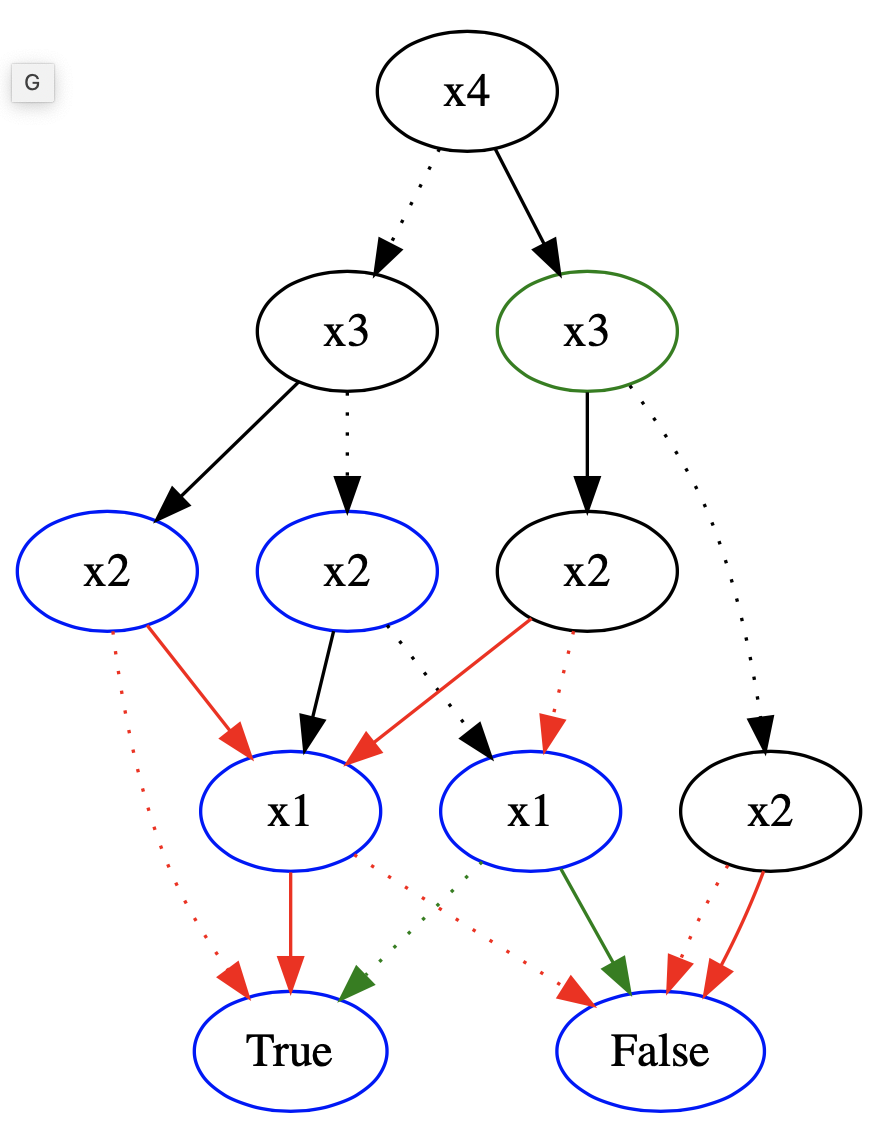
\includegraphics[scale=0.35]{tree21_new.png}
    \caption{Dag}
    \label{fig:tree21_new}
\end{figure}
On considère la figure \ref{fig:tree21_new}. Les pointeurs sont représentés en rouge. Le squelette du robdd est le graphe réduit aux transitions en noirs.

La pool du noeud entouré en vert est : \(\{x_2,x_2,x_1,x_1,\top,\bot\}\). 

Le profil de ce bdd est : \{2,2,4,2,1\}.

\vspace{5mm} 

Nous savons de la manière dont nous définissons les bdd que pour être valide un bdd \(\beta\) doit avoir les propriétés suivantes:

FACT 1.1 : \emph{De la règle r nous faisons la conclusion que deux noeuds de même index ne peuvent avoir les même descendants, autrement ils auraient été fusionnés.}

FACT 1.2 : \emph{A partir de la règle m nous savons qu'un noeud ne peut avoir deux enfants identiques, autrement ce noeud aurait été supprimé.}

\section{Comptage}
La méthode classique permettant d'énumérer les bdd ayant un nombre de variable k et une taille n est la suivante:
\begin{enumerate}
    \item 
	Énumérer toute les \({2^2}^k\) fonctions booléennes et dresser leurs arbres de décision binaires
	\item
	Appliquer le processus de compression pour obtenir leur bdd
	\item
    Filtrer les bdd de taille n
	\item
	Supprimer les bdd réapparaissant plus d'une fois afin de ne conserver qu'une seule de leur occurrence
\end{enumerate}
Nous proposons ici une méthode récursive permettant d'effectuer cette énumération sans passer ni par le processus de compression ni celui du filtrage. Ces deux processus sont hautement coûteux avec une complexité doublement exponentielle \(O(2^{2^{k}})\).
\vspace{5mm} 

\textbf{Proposition 1} :  Considérons T = (Q’, I, r, \(\delta\)’) un squelette avec un ensemble de noeuds Q’, racine r et fonction de transition partiel \(\delta\)’ : Q’ \(\times\) \{0, 1\} \(\rightarrow\) Q’ \(\cup\) \{nil\}. La fonction de transition entière \(\delta\) : Q’ \(\times\) \{0, 1\} \(\rightarrow\) Q’ \(\cup\) \{\(\top\), \(\bot\)\} est la fonction de transition d'un bdd avec un squelette T si et seulement si pour tout noeuds \(\lambda\) \(\in\) Q’, noté \(\lambda\)0 = \(\delta\)(\(\lambda\), 0) et \(\lambda\)1 = \(\delta\)(\(\lambda\), 1), la paire (\(\lambda\)0, \(\lambda\)1) satisfait : 
\begin{enumerate}
    \item 
	Si \(\delta\)’(\(\lambda\), 0) != nil et \(\delta\)’(\(\lambda\), 1) != nil alors 
	\begin{center}
	\(\lambda\)\(\sigma\) = \(\delta\)’(\(\lambda\), \(\sigma\)) pour \(\sigma\) \(\in\) \{0, 1\}.
    \end{center}
    \item
	Si \(\delta\)’(\(\lambda\), 0) = \(\delta\)’(\(\lambda\), 1) = nil, alors 
	\begin{center}
	\(\lambda\)\(\sigma\) \(\in\) PT(\(\lambda\))  pour \(\sigma\) \(\in\) \{0, 1\} et \(\lambda\)0 != \(\lambda\)1, et il n'y a aucun noeud \(\lambda\)’ != \(\lambda\) avec I(\(\lambda\))=I(\(\lambda\)’) tel que \(\delta\)(\(\lambda\)’, ·) = \(\delta\)(\(\lambda\), ·).
    \end{center}
    \item
	Si \(\delta\)’(\(\lambda\), 0) = nil et \(\delta\)’(\(\lambda\), 1) != nil, alors
	\begin{center}
	\(\lambda\)0 \(\in\) PT(\(\lambda\)) et \(\lambda\)1 = \(\delta\)’(\(\lambda\), 1).
	\end{center}
    \item
	Si \(\delta\)’(\(\lambda\), 0) != nil et \(\delta\)’(\(\lambda\), 1) = nil, alors 
	\begin{center}
	\(\lambda\)0 = \(\delta\)’(\(\lambda\), 0) et \(\lambda\)1 \(\in\) PT(\(\lambda\)) \(\cup\) TA(\(\lambda\)0) \(\setminus\) \(\lambda\)0 .
    \end{center}
\end{enumerate}
\newpage
Preuve. Puisque \(\delta\)(·, ·) doit étendre \(\delta\)’(·, ·), le cas 1. est triviale. En effet, nous devons étendre la fonction de transition uniquement lorsque l'on a \(\delta\)(\(\lambda\), \(\sigma\)) = nil. Dans le cas 2., nous devons choisir pour (\(\lambda\)0, \(\lambda\)1) deux noeuds dans PT(\(\lambda\)). De plus \(\lambda\)0 != \(\lambda\)1 comme déclaré dans FACT 1.2 et un autre noeud avec le même index que \(\lambda\) ne peut pas avoir les même enfants (\(\lambda\)0, \(\lambda\)1) comme déclaré dans FACT 1.1. Dans le cas 3., l'enfant bas doit être choisi dans la pool de \(\lambda\) puisque l'on doit préserver le squelette. Dans le cas 4., l'enfant haut de \(\lambda\) est aussi choisi dans la pool de  \(\lambda\) ou dans TA(\(\lambda\)0) (et doit être diffèrent de \(\lambda\)0).
\vspace{5mm} 

Nous définissons maintenant un procédé permettant de calculer le nombre de bdd correspondant à un squelette donné, nous appellerons le nombre de bdd correspondant à un squelette S le poids de S.

\textbf{Poids d'un noeud} : Considérons un squelette T = (Q’, I, \(\delta\)’, r), le poids wT(\(\lambda\)) d'un noeud \(\lambda\) \(\in\) Q’ est le nombre de transitions possibles pour compléter la fonction de transitions partielles \(\delta\)’(\(\lambda\), ·) et former un bdd valide de squelette T.

\textbf{Proposition 2} (Poids d'un noeud) : Considérons T = (Q’, I, \(\delta\)’, r) un squelette , le poids wt(\(\lambda\)) d'un noeud \(\lambda\) \(\in\) T est:

\begin{equation}
    wt(\lambda) =
    \begin{cases}
        1 & \text{si \(\delta\)’(\(\lambda\), 0) != nil et \(\delta\)’(\(\lambda\), 1) != nil}\\
        pts(\lambda) (pts(\lambda) - 1) - ST(\lambda) & \text{si \(\delta\)’(\(\lambda\), 0) = \(\delta\)’(\(\lambda\), 1) = nil}\\
        pts(\lambda) + pts0(\lambda) - 1  & \text{si \(\delta\)’(\(\lambda\), 0) = nil et \(\delta\)’(\(\lambda\), 1) != nil}\\
        pts(\lambda)   & \text{si \(\delta\)’(\(\lambda\), 0) != nil et \(\delta\)’(\(\lambda\), 1) = nil}
    \end{cases}       
\end{equation}

Avec pts(\(\lambda\)) = \(\mid\mid profil(PT(\lambda)) \mid\mid\) et pts0 = \(\mid\mid profil(TA(\delta \textquoteright(\lambda,0))) \mid\mid\).

Preuve. A partir de la proposition 1 nous énumérons tous les liens possibles (liant à un noeud) nous pouvons utiliser pour compléter la fonction de transition partielle. Dans le premier cas nous ne pouvons compléter que avec les liens déjà existant (comme déclaré dans 1) de proposition 1) le cas est déjà défini). Dans le second cas nous énumérons tous les liens possible de 2) de la proposition 1. Dans le troisième et quatrième cas nous faisons la même chose pour respectivement  3) et 4).
\vspace{5mm} 

Le poids d'un sous arbre est le poids cumulé de ses noeuds.

\textbf{Poids d'un squelette} : Considérons un squelette T = (Q’, I, \(\delta\)’, r), le poids W(T) de T est le poids cumulé de ses noeuds.
\[W(T) = \prod wt(\lambda) \mid \lambda \in Q\textquoteright\]


Dans le cas où le poids d'un noeud \(\lambda \in Q\textquoteright\) est nul ou négative nous savons que le squelette T est invalide parce que T n'est le squelette d'aucun BDD. Ceci arrive uniquement lorsque \(\lambda\) a ses deux enfants égaux à nil (puisque l'on a nécessairement \(\mid\mid profil(PT(\lambda)) \mid\mid \geq\)2).

Cette formule peut être aisément décrite de manière récursive, via une traversée en \(post_{o}\) où toutes les informations nécessaires pour calculer le poids du noeud ont déjà été traitées.
\vspace{5mm} 

Nous notons \(T_{nk}\) l'ensemble des squelettes de taille n et de nombre de variables k, et \(N_{nk}\) le nombre de bdd de taille n et de nombre de variables k.
Pour déterminer \(N_{nk}\) tout ce que nous avons à faire est déterminer la totalité des squelettes de taille n et de nombre de nombre de variables k et ensuite déterminer leurs poids, nous les additionnons par la suite.

\[N_{nk} = \sum W(T) \mid T \in T_{nk}\]

\section{Combinatoire sur les squelettes}
Ce que nous voulions dans la section précédente était d'énumérer tout les bdd de taille n et de nombre de variables k. Pour ce faire nous devons déterminer les squelette de taille n et de nombre de variable k. Il ne s'agit pas d'un processus aisé à informatiser.

Nous définissons ici un processus récursif où nous construisons les squelettes à l'aide de chacun des noeuds composant ceux-ci et dès lors que l'on a déterminé qu'un squelette n'est pas valide on l'ignore. 
\vspace{5mm} 

Nous définissons un squelette Tt en tant que tuple tel que:
$Tt=T' \cup N_i \cup T''| nil$ 
%\[Tt = T\textquoteright \cup N_i \cup T\textquoteright\textquoteright \mid nil \]
où \(N_i\) est un noeud d'index i. Ceci signifie que le squelette est soit réduit à nil soit à une racine et deux squelette. Nous désignerons dans la suite les squelette T' et T'' qui composent Tt par le terme de sous squelette.

Pour considérer un squelette enraciné en r en particulier nous prendrons en compte trois de ses paramètres. Sa pool pT(T), le level rank de sa racine ST(r) et sa taille que nous désignerons par \(\mid\mid T\mid\mid\).

Ces paramètres sont fondamentaux pour déterminer le poids des squelettes considérés.

Nous utiliserons la notation \(T_{m,p,s} \) pour considérer le squelette enraciné en r de taille m (m =  \(\mid\mid T\mid\mid\)), de pool profil p (p = profil(pT(r))) et de level rank s (s = ST(r)) représenté par un tuple Tt tel décrit plus haut.


\textbf{Proposition 3} :  Pour \(T_{m,p,s} \) nous considérons des tailles pour chaque sous squelette T’ \(\cup\) T’’ \(\in\) T de respectivement i et m – 1 – i, avec \(0\leq i\leq m-1\). Pour chacune des tailles de sous squelette considérée, nous déterminons chacune des valeurs d'indexs que l'on peut assigner à leur racine.

Nous avons ainsi un algorithme dans lequel nous considérons toute les tailles possible ainsi que les indexes des sous-squelette, le level rank de la racine étant déjà donné par le pool profil du squelette courant (ainsi que par le profil de T' dans le cas du level rank de T''). k correspond dans la suite à la taille de p.

\begin{enumerate}
    \item Si m>0
        \begin{enumerate}
            \item
            \(T\textquoteright \in \underset{k_0\in K}{\bigcup} T_{i,p[:k_0-1],p_{k_0-1}} \)
            \item
            \(T'' \in \underset{k_0\in K}{\bigcup} T_{j,p1[:k_0-1],p1_{k_0-1}} \)
            %\(T\textquoteright\textquoteright \in \underset{k_0\in K}{\bigcup} T_{j,p1[:k_0-1],p1_{k_0-1}} \)
            \item
            $WTP(N_k,T',T'')*W(T')*W(T'')$
            %\(W(T)=WTP(N_k,T\textquoteright,T\textquoteright\textquoteright)*W(T\textquoteright)*W(T\textquoteright\textquoteright)\)
        \end{enumerate}
 
    \item Si m = 0
        \begin{enumerate} 
            \item
            T=nil 
            \item
            W(T)=1
        \end{enumerate}
\end{enumerate}
Avec j = m-1-i, on note p[:i]=(\(p_0,p_1...p_i\)) pour designer dans un ensemble p que l'on ne considère que les éléments ayant un index plus petit ou égal à i et \(p_{k}\) lorsqu'on désigne l'élément d'index k. On a également p1=p+profil(TA(T')) et K = \{0,1,...,k\}. Enfin on note W(T) le poids du squelette T et WTP(N,T',T'') le poids du noeud N qui a pour fils bas le squelette T' et pour fils haut le squelette T''.
\vspace{5mm} 

Avec notre algorithme, nous ne considérons, pour chaque récursion, uniquement les squelettes ayant les même valeurs m, p et s. 
En s'inspirant de ce procédé on peut écrire un algorithme COUNT(m,p,s) prenant en argument une taille de squelette m, un profil p et un level rank s et retournant un dictionnaire au sein duquel chaque clé est le profil d'un squelette, et la valeur, la somme des poids des squelettes ayant ce profil. 

Quelques exemples d'exécution de la fonction COUNT:
\begin{itemize}
    \item COUNT(3,(2,0,0),0) nous retourne \{(0,1,1,1): 56, (0,2,0,1): 2, (0,0,2,1): 2\}
    \item COUNT(2,(2,0),0) nous retourne  \{(0,1,1): 8\}
    \item COUNT(1,(2),1) nous retourne \{(0,1): 1\}
\end{itemize}

Dans le premier cas le dictionnaire retourné nous indique qu'il existe 56 squelette unique de taille 3 ayant pour profil (0,1,1,1), 2 ayant pour profil (0,2,0,1) et encore 2 ayant pour profil (0,0,2,1).

\vspace{5mm} 

S'appuyant sur l'algorithme COUNT on définit N(n,k) qui renvoie le nombre de bdd de taille n et d'index k:
\[N(n,k)=\underset{(t,w)\in COUNT(n-2,(2,0,...,0),0)}{\sum} w\]

\(e^{(k)}\) est une liste de k+1 composants tous nuls sauf le dernier qui est égal à 1 tel que \(e^{(k)} = (0,0,...,1)\).

La complexité de l'algorithme COUNT est exponentiel de l'ordre de \(O(2^{3k^2/2+k})\).

L'algorithme COUNT s'appuie sur la méthode de comptage et de génération des squelettes que l'on a décrit plus haut. Cet algorithme vérifie tout d'abord si le noeud courant est vide (m=0). Si tel est le cas, on sait qu'on est sur une nil-transition. Si le noeud courant n'est pas vide (m>0) on génère la totalité des sous arbres gauche et droit et déterminons récursivement leurs poids. Nous stockons leur poids dans un dictionnaire selon leurs profil.
\begin{algorithm}
  \begin{algorithmic}[1]
    \Statex
    \Function{COUNT}{m,p,s}
      \State \Let{$d\gets \{\}$}
      \State \Let{$k\gets $Len(p)-1} \Comment{Len(p): renvoie la taille de la liste p}
      \If{m=0}
        \State \Let{$S\gets (\sum_{k-1}^{j=0} p_j)(\sum_{k-1}^{j=0} p_j-1)$}
        \If{$S>0$}
            \State \Let{$d \gets \{e^{(k)}:S\}$}
        \EndIf
      \Else
        \For{$i \gets$ 0 to m$-1$}
            \State \Let{$d_0\gets \{\}$}
            \If{i=0}
                \Let{$d_0 \gets \{():\sum_{k-1}^{i=0} p_i\}$}
            \Else
                \For{$k_0 \gets$ 1 to $k-1$}
                    \Let{$d_0 \gets d_0 \cup $COUNT$(i,p[:k_0-1],p_{k_0})$}
                \EndFor
            \EndIf
            \For{$(l,w_0) \gets d_0$}
                \State \Let{$d_1\gets \{\}$}
                \State \Let{$p\textquoteright \gets p+l$}
                \If{n-1-i=0}
                    \Let{$d_1 \gets \{():-1+\sum_{k-1}^{i=0} p_i\textquoteright\}$}
                \Else
                    \For{$k_1 \gets 1$ to $k-1$}
                        \State \Let{$d_1 \gets d_1 \cup $COUNT$(n-1-i,p'[:k_1-1],p'_{k_1})$}
                    \EndFor
                \EndIf
                \For{$(r,w_1) \gets d_1$}
                    \State \Let{$w \gets w_1*w_0$}
                    \State \Let{$t \gets l+r+e^{k}$}
                    \If{$t\in d$}
                        \Let{$d[t] \gets d[t]+w$}
                    \Else
                        \Let{$d \gets d \cup \{t:w\}$}
                    \EndIf\EndFor\EndFor\EndFor\EndIf
      \State \Return{$d$}
    \EndFunction
  \end{algorithmic}
\end{algorithm}

\newpage
\section{Unranking}
Notre approche pour le unranking s'appuie sur la méthode introduite dans \cite{wilf} où l'on décompose un arbre binaire en ses sous arbre gauche et droits et en attribuant à chaque décomposition un ordre total pour un bdd de taille et d'index fixé.

En s'inspirant de la Proposition 3 on définie une méthode récursif b permettant de déterminer le nombre d'arbres binaires ayant une certaine taille n.

\begin{equation}
    b_n =
    \begin{cases}
        1 & \text{si n = 0}\\
        \sum_{k=0}^{n-1}b_k*b_{n-1-k}  & \text{sinon}\\
    \end{cases}      
\end{equation}

En s'appuyant sur cette méthode on peut definir une decomposition sur un arbre de taille fixé n. Cette méthode s'appuie sur le fait que \(b_n\) est définie en une somme de produit, où chaque élément du produit peut être vu comme la repreésentation d'un arbre ayant un sous arbre gauche et un sous arbre droit de taille fixe. Par exemple \(B_7\) = 429, et on peut le décomposer en:
\[B_7=B_0*B_6+B_1*B_5+B_2*B_4+B_3*B_3+B_4*B_2+B_5*B_1+B_6*B_0\]
\[429=1*132+1*42+2*14+5*5+14*2+42*1+132*1\]

Où \(B_2*B_4\) représente un arbre composé d'un sous arbre droit de taille 4 et d'un sous arbre gauche de taille 2.

Ainsi, si je cherche l'arbre n\si{\degree}250 de taille 7, j'obtiens : 250 = 132 + 42 + 28 + 25 + 23. On trouve donc que l'arbre 250 est composé d'un enfant gauche de taille 4 et d'un enfant droit de taille 2. Et plus particulièrement, parmi les 28 arbres ayant cette décomposition 4x2, c'est l'arbre numéro 23 qui nous intéresse.


Pour ensuite retrouver le numéro des sous arbre gauche et droit on procède comme ceci:
\begin{itemize}
    \item 23 //\( B_2 \) pour le numero du sous arbre gauche
    \item 23 \% \(B_2\)   pour le numero du sous arbre droit
\end{itemize}

En s'appuyant recursivement sur cette methode, on obtient l'arbre de la figure \ref{fig:generation d'arbre}.

\begin{figure}[htp]
    \centering
    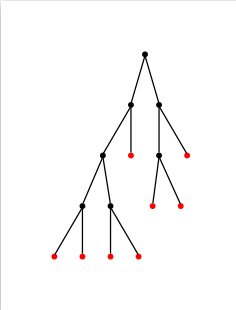
\includegraphics[width=3cm, height=4cm]{tree generation.png}
    \caption{Arbre de taille 7 et de rang 250 généré}
    \label{fig:generation d'arbre}
\end{figure}

En s'inspirant de cette même méthode, on peut définir une fonction DECOMPOSE(r\textquoteright,n\textquoteright,s,p\textquoteright) permettant de générer un bdd de taille n\textquoteright, ayant un profil p\textquoteright et un rang r\textquoteright. s est une variable contenant le squelette du bdd a générer.

\begin{algorithm}
  \begin{algorithmic}[1]
    \Statex
        \Function{decompose}{$rank, n, squelette, p$}
            \State \Let{$p\_target \gets $list$(p)$} 
            \State \Let{$r \gets rank$}
            \State \Let{$s \gets squelette.$get\_profil$()$}
            \State \Let{$k \gets $len$(p\_target)-1$}
            \State \Let{$q \gets s[:k]$}
            \State \Let{$q[0] \gets 2$}
            \State \Let{$i \gets  n-1$}
            \While{$i \geq 0$}
                \If{$i = 0$}
                    \State \Let{$d0 \gets {(): $sum$(q,1,k-1)+2}$}
                \Else
                    \State \Let{$d0 \gets \{\}$}
                    \For{$k0 \gets $range$(1,k)$}
                        \State \Let{$d0.$update$($count$(i,q[:k0],q[k0]))$}
                    \EndFor
                \EndIf
                \For{$(l,w0)$ in $d0.$items$()$}
                    \State \Let{$q\_prim \gets $sum\_profil$(q,l) $}
                    \If{$n-1-i = 0$}
                        \State \Let{$d1 \gets \{():$sum$(q\_prim,1,k-1)+1\}$}
                    \Else
                        \State \Let{$d1 \gets \{\}$}
                        \For{$k1$ in range$(1,k)$}
                        \State \Let{$d1.$update$($count$(n$-$1$-$i,q\_prim[:k1],q\_prim[k1]))$}
                        \EndFor
                    \EndIf
                    \For{$(h,w1)$ in$ d1.$items$()$}
                        \State \Let{$t \gets $sum\_profil$($sum\_profil$($e\_k$(k),$list$(l)),$list$(h))$}
                        \State \Let{$w \gets w0*w1$}
                        \If{$t = p\_target$}
                            \If{$w > 0$}
                                \State \Let{$r \gets r - w$}
                            \EndIf
                            \If{$r < 0$}
                                \State \Let{$r  \gets r + w$}
                                \State \Let{$r0 \gets r \% w0$}
                                \State \Let{$r1 \gets r // w0$}
                                \State \Return{$(i,r0,l,r1,h)$}
                            \EndIf
                        \EndIf
                    \EndFor
                \ENDFOR
                \State \Let{$i \gets i - 1$}
  \end{algorithmic}
\end{algorithm}
\newpage

On décrit ensuite une fonction GENERATE(r,n,s,p) permettant de générer un squelette de taille n, de profil p et de rang r. La variable s est une variable globale qui contiendra en fin d'exécution le bdd généré.
Cette fonction prend en argument un squelette s contenant les noeuds initialement dans la pool (ici \(\up\) et \(\bot\)) et crée au fur et a mesure le bdd souhaité en faisant appel à la fonction décompose et en mettant à jour le squelette.

\begin{algorithm}
  \begin{algorithmic}[1]
    \Statex
        \Function{generate}{$rank, n, squelette, p\_target$}
            \State \Let{$k \gets $len$(p\_target)-1$}
            \If{$n = 0$}
                \State \Let{$node \gets squelette.$unrank\_singleton$(rank)$}
                \State \Return{$ node$}
            \EndIf
            \If{$n = 1$}
                \Let{$lo,hi \gets squelette.$unrank\_pair$(rank,k)$}
            \Else
                \State \Let{$i,r0,l,r1,h \gets $DECOMPOSE$(rank,n,squelette,p\_target)$}
                \State \Let{$lo \gets $GENERATE$(r0,i,squelette,l)$}
                \If{$n-1-i=0$}
                    \Let{$hi.$unrank\_singleton$(r1)$}
                        \If{$hi=lo$}
                            \Let{$hi \gets $GENERATE$(r1-1, n-1-i, squelette, h)$}
                        \EndIf
                    \Else
                        \State \Let{$hi \gets $GENERATE$(r1, n-1-i, squelette, h)$}
                \EndIf
            \EndIf
            \State \Let{$node \gets squelette.$add\_node$(rank,k,lo,hi)$}
            \State \Return{$node$}
  \end{algorithmic}
\end{algorithm}


Dans la fonction GENERATE on fait en sorte d'identifier les noeuds que l'on peut assigner aux nil-transitions du noeud courant. Pour un noeud v ayant deux nil-transitions on vérifie donc avant de lui assigner en tant que haut fils un noeud n et fils bas un noeud m que I(m)<I(v) et I(n)<I(v), on vérifie également qu'il n'existe pas v\textquoteright \(\in\) squelette tel que v!=v\textquoteright, où v\textquoteright a pour fils bas m\textquoteright et pour fils haut n\textquoteright, que m=m\textquoteright et n=n\textquoteright.

On fait ensuite de même lorsque le noeud courant a une seul nil-transitions en tant que fils bas ou en tant que fils haut tout en respectant les règles que l'on a déjà décrit pour la génération des bdd. 

Pour cela on utilise ces fonctions:
\begin{itemize}
    \item unrank\_singleton(r) : cette fonction retourne un noeud compatible avec le noeud courant de rang r.
    \item unrank\_pair(rank, k) : Cette fonction retourne une pair de noeud dont l'index est strictement inférieur à k, on omet également les pair de noeuds déjà assignés en tant que descendant d'un noeud précèdent de même index.
    
%    \item  get\_rank(i) : Cette fonction retourne le noeud de rang i compatible avec le noeud courant.
%    \item get\_profil() : Cette fonction retourne retourne le profil du squelette courant.
% On a pas l'air d'utiliser ces deux la???
    \item add\_node(lo, hi, k): Cette fonction crée le noeud d'index k et ayant pour descendants bas et haut lo et hi.
\end{itemize}

\newpage
Enfin on décrit une fonction GEN\_BDD(r,n,k) permettant de générer un bdd de taille n, d'index k et de rang r en utilisant la fonction GENERATE décrite précédemment.

\begin{algorithm}
  \begin{algorithmic}[1]
    \Statex
        \Function{gen\_bdd}{$rank, n, k$}
            \State \Let{$squelette \gets $Squelette$(k)$}
            \State \Let{$r    \gets rank$}
            \State \Let{$p    \gets [0]*k$}
            \State \Let{$p[0] \gets 2$}
            \State \Let{$d \gets $count$(n-2,p,0)$}
            \For{$(t,w)$ in $d.$items$()$}
                \State \Let{$r \gets r - w$}
                \If{$r < 0$}:
                    \State \Let{$r \gets r + w$}
                    \State \Let{generate$(r,n-2,squelette,t)$}
                    \State \Return{$squelette$}
            \EndFor
  \end{algorithmic}
\end{algorithm}

Squelette est ici une classe d'objet permettant de représenter un squelette. Voir Annexe \ref{Annexe_1} pour une représentation en python de la classe squelette.

La méthode du unranking nous permet de mettre au point un générateur aléatoire uniforme de bdd.

\begin{figure}[h!]
    \centering
    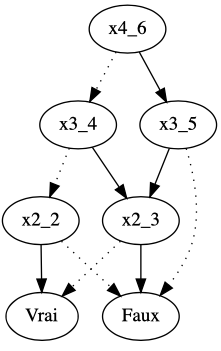
\includegraphics[scale=0.4]{arb_3104.png}
    \caption{Graphe(A) rang = 3104}
    \label{fig:graphe_A}
\end{figure}
L'ensemble dans lequel on a choisi le squelette du graphe(A) de la figure \ref{fig:graphe_A} est : \{(0, 2, 1, 1, 1): 584, (0, 1, 2, 1, 1): 1256, (0, 2, 2, 0, 1): 74, (0, 1, 1, 2, 1): 1112, (0, 2, 0, 2, 1): 74, (0, 0, 2, 2, 1): 74\}.

Avec un rang=3104, on déduit le profile du squelette du graphe est (0, 0, 2, 2, 1). Puisqu'en faisant la somme 584+1256+74+1112+74 = 3100, on remarque que l'on a pas atteint 3104, le seul choix possible reste le dernier.

Avec un rang=3104 et le profile de squelette généré on se retrouve avec {x1=0 ; x2=2  ; x3=2; x4 = 1} et le graphe de la figure \ref{fig:graphe_A}.

\section{Tests Quickcheck}

\subsection{Combinaison de BDD(fonction melding)}
Melding fonction est une combinaison de deux BDD, dont le résultat est la conjonction logique ET. Cette fonction que nous utilisons provient de l'ouvrage de KNUTH \cite{knuth}. Le code consiste à combiner les deux BDD en comparant les indexes de noeuds, pour deux noeuds de même index, en résulte un noeud commun. le BDD 
(C ~\ref{fig:graphe_C}) est une combinaison(melding) des BDD (A ~\ref{fig:graphe_A}) et (B ~\ref{fig:graphe_B}).

\begin{figure}[h!]
    \centering
    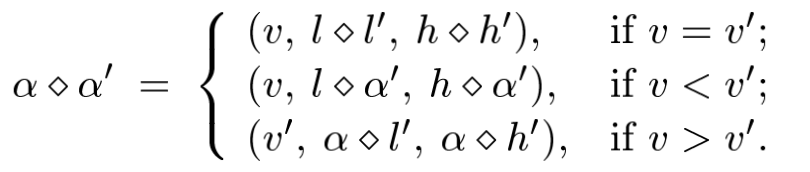
\includegraphics[scale=0.5]{melding_formula.png}
    \caption{Combinaison de $\alpha(v,l,h)$ et $\alpha'(v',l',h')$}
    \label{fig:melding_formula}
\end{figure}

\begin{figure}[h!]
    \centering
    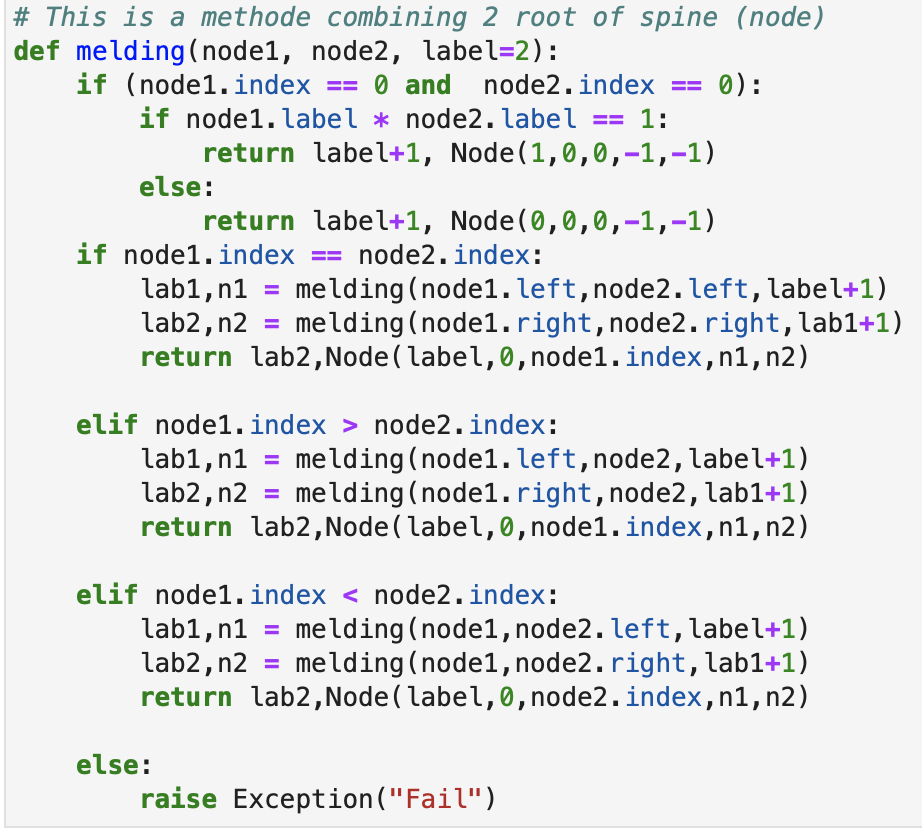
\includegraphics[scale=0.6]{melding_function.png}
    \caption{fonction melding}
    \label{fig:melding_function}
\end{figure}


\subsection{Stratégie de Test}
Dans nos tests, nous utilisons \href{https://github.com/HypothesisWorks/hypothesis}{Quickcheck pour python}. Nous intégrons notre générateur dans des tests Quickcheck.\newline

\begin{figure}[h!]
    \centering
    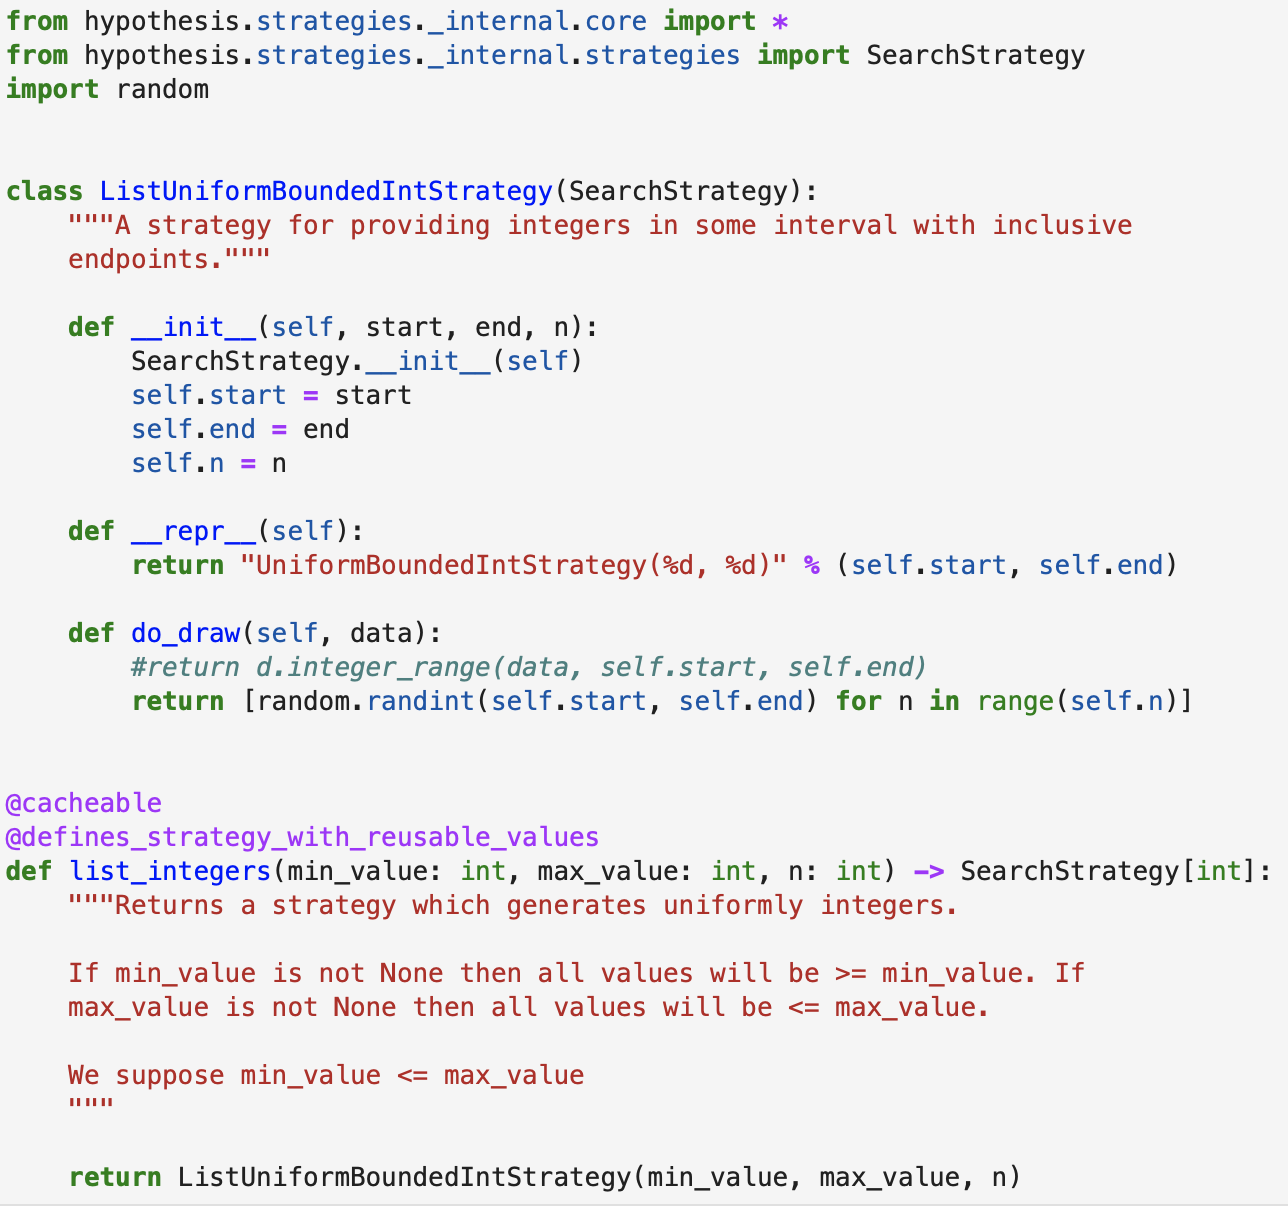
\includegraphics[scale=0.4]{geration_uniform.png}
    \caption{génération uniforme d'entiers}
    \label{fig:geration_uniforme}
\end{figure}

À partir d'un ensemble de 10 entiers générés uniformément\ref{fig:geration_uniforme}, nous construisons un ensemble BDD
Pour chaque couple (A,B) de cet ensemble nous les combinons avec la fonction fonction melding pour
obtenir un BDD C. Pour une confirmation du test nous comparons les tables de vérités des BDD {A,B,C}  par la formule suivante : table(A) ET(logique) table(B) égal à table(C) \ref{fig:test_rank}.

\begin{figure}[h!]
    \centering
    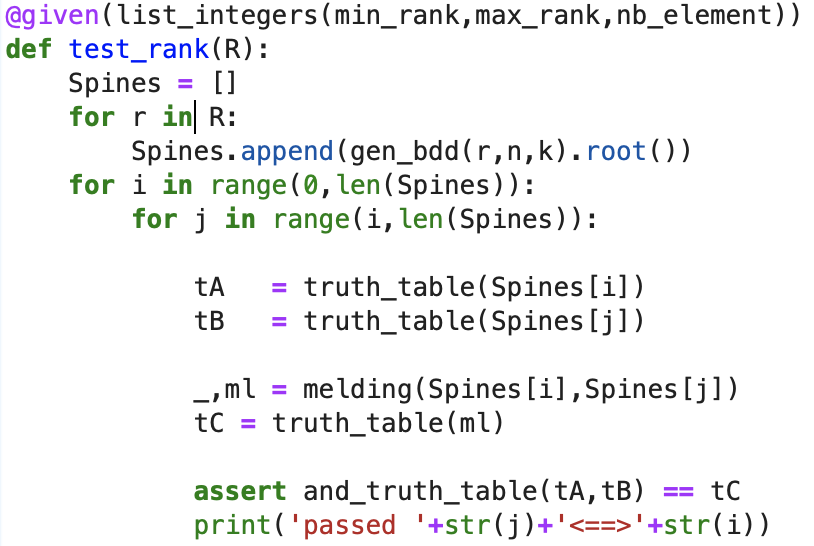
\includegraphics[scale=0.4]{test_rank.png}
    \caption{Tests des tables de vérités}
    \label{fig:test_rank}
\end{figure}

\begin{figure}[h!]
    \centering
    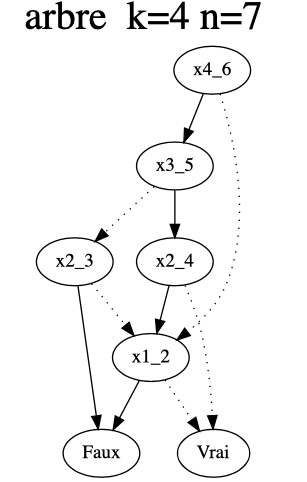
\includegraphics[scale=0.4]{arb_1577.png}
    \caption{BDD(B) rang(rank) = 1577}
    \label{fig:graphe_B}
\end{figure}

\begin{figure}[h!]
    \centering
    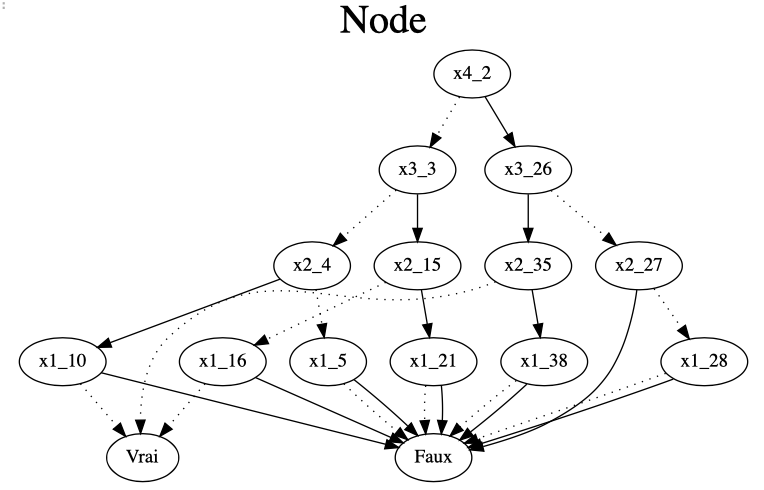
\includegraphics[scale=0.4]{abr_melding_C.png}
    \caption{BDD(C) combinaison(melding) de A et B}
    \label{fig:graphe_C}
\end{figure}


\section{Conclusion}
Il ne fait aucun doute que la méthode présenté dans ce rapport offre un gain en temps et en espace gigantesque pour la résolution du problème présenté, la génération de bdd. Nous avons vu que même avec un matériel limité, nous pouvions générer un grand nombre de bdd en un temps record. Ce qui n'était pas possible avec la méthode standard. 

Cette génération en plus de sa simplicité, présente d'autres gains tels que la possibilité de l'adapter selon nos besoins. Nous pouvons ainsi l'adapter pour pouvoir générer d'autre types d'arbre de décisions.
Mais comme nous l'avons vu ce gain ne se limite pas a la seule génération de bdd. Cette méthode offre une toute nouvelle manière d'appréhender ainsi que que de nouveaux moyens d'études des Binary Decision Diagram.

On note également que l'on pourrait encore améliorer notre méthode, par exemple en faisant en sorte de ne considérer que les bdd valides, ou en améliorant le processus de comptage. 
\newpage
\section{Annexe}
\subsection{Annexe 1}
\label{Annexe_1}
Description en python de la classe squelette. 

\begin{figure}[H]
    \centering
    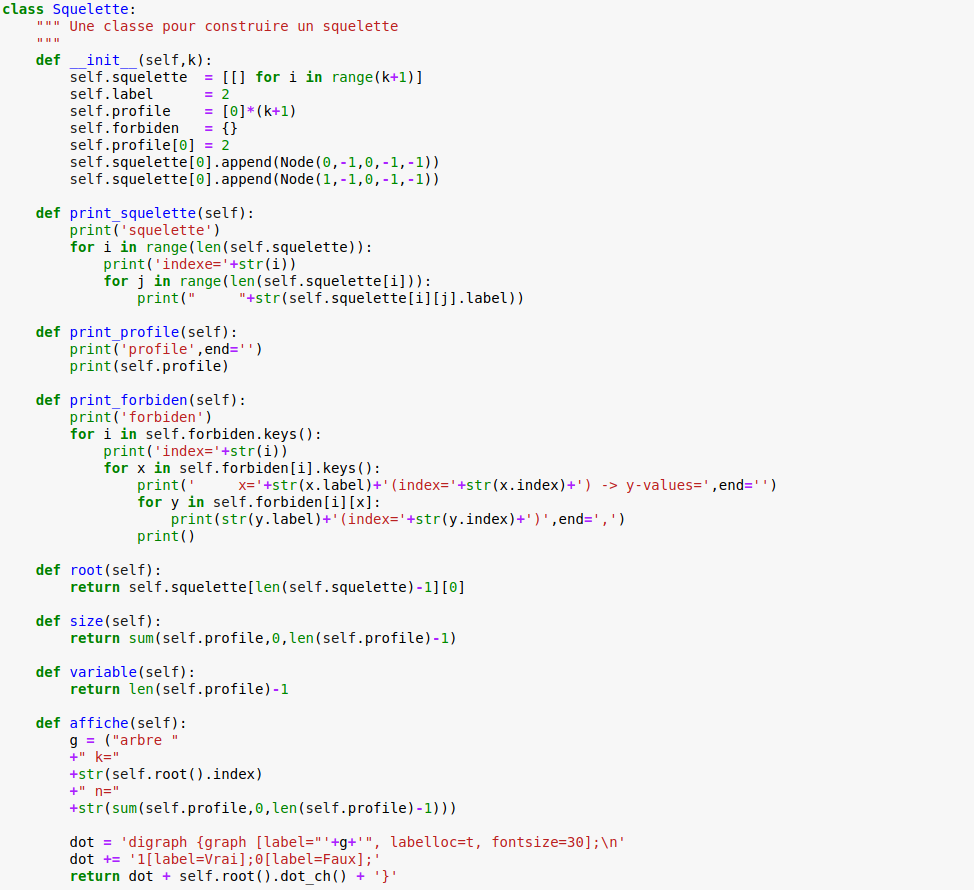
\includegraphics[scale=0.4]{part1_squelette.png}
    \caption{partie 1 classe squelette}
    \label{fig:squelette1}
\end{figure}

\begin{figure}[H]
    \centering
    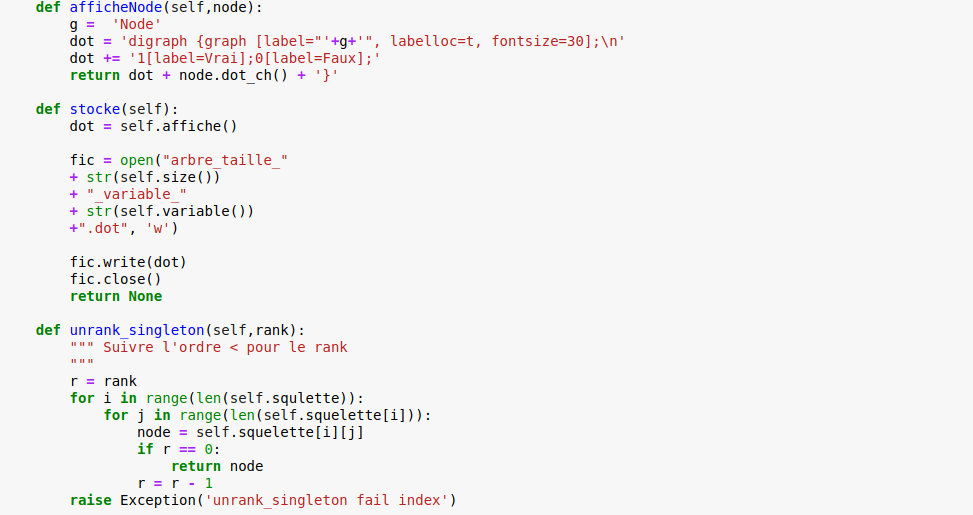
\includegraphics[scale=0.4]{part2 squelette.png}
    \caption{partie 2 classe squelette}
    \label{fig:squelette2}
\end{figure}

\begin{figure}[H]
    \centering
    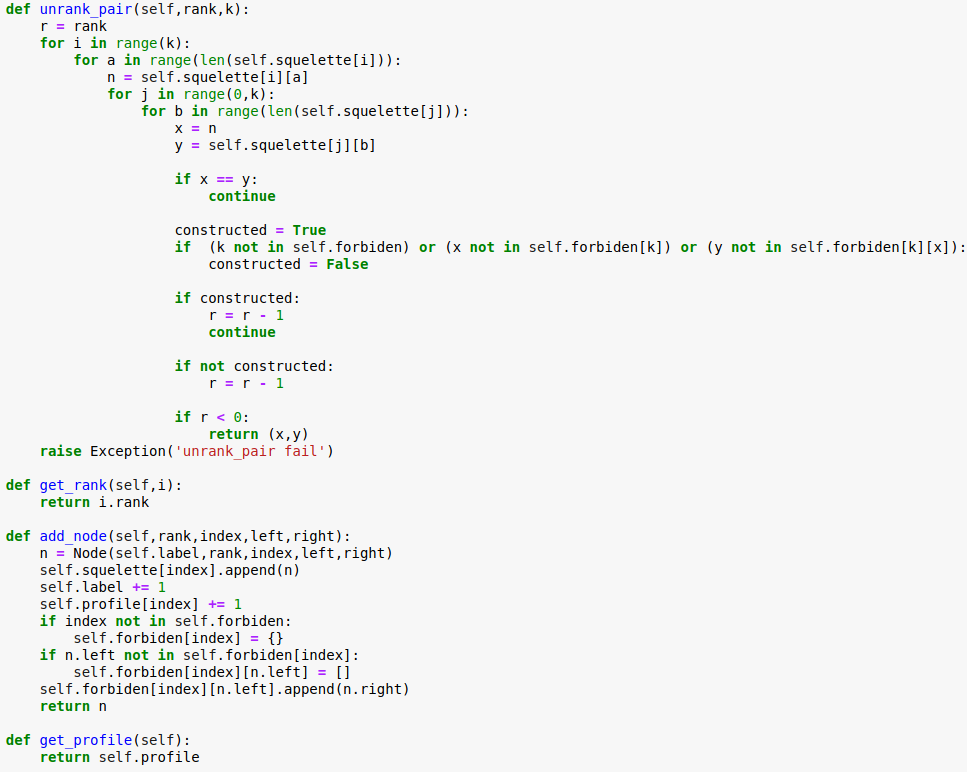
\includegraphics[scale=0.4]{part3 squelette.png}
    \caption{partie 3 classe squelette}
    \label{fig:squelette3}
\end{figure}




\newpage
\addcontentsline{toc}{section}{References}
\printbibliography

\end{document}
